\documentclass[10pt,a4paper]{article}

\usepackage{geometry}
\geometry{a4paper, top=30mm, left=30mm, right=30mm, bottom=30mm,
headsep=10mm, footskip=12mm}
\usepackage[utf8]{inputenc}
\usepackage[ngerman]{babel}
\usepackage[T1]{fontenc}
\usepackage{lmodern}
\usepackage{graphicx}
\usepackage{wrapfig}
\usepackage{pdfpages}
\usepackage{longtable}
\usepackage{enumerate}
\usepackage{enumitem}
\usepackage{wasysym}
\usepackage{amssymb}




\usepackage[footsepline,headsepline]{scrpage2}
\pagestyle{scrheadings}
\ohead{\thetitle}
\ihead{Team: jupleg}
\ofoot{Seite \thepage}
\cfoot{} % if left empty, removes page number at center
\title{Projekt}
\author{Team: jupleg}



\begin{document}
\maketitle
\newcommand{\thetitle} {Projekt}

\section*{Quälgeist}
\begin{itemize}
\item Was macht das Programm:\\
Es ist eine Erweiterung/ Abwandlung vom Brettspiel Cluedo.\\
Kind (Quälgeist) hat den Mord an der Putzfrau im Haus seiner Eltern beobachtet und Du als Ermittler musst den Mord aufklären.\\
Das Kind hat Hinweise, will diesen aber nicht teilen. Um diese doch zu bekommen musst Du Aufgaben erledigen, die das Kind (der Quälgeist) stellt. Aber Achtung, es will nicht immer helfen und manchmal haut es dir ab.\\
Wenn Du eine Vermutung hast, dann kannst Du diese äußern. 
Wenn Du aber dreimal eine falsche Verdächtigung gemacht hast, dann verlierst Du deinen Job und auch das Spiel.\\
\ \\
Mögliche Täter:
\begin{itemize}
\item Vater
\item Mutter
\item Gärtner
\item Koch
\item Nachbar
\item Besuch
\end{itemize}
Mögliche Tatorte:
\begin{itemize}
\item Eingangsbereich
\item Schlafzimmer
\item Küche
\item Garten
\item Wohnzimmer
\item Arbeitszimmer
\end{itemize}
Mögliche Tatwaffen:
\begin{itemize}
\item Pistole
\item Messer
\item Seil
\item Spaten
\item Gift
\item Pokal
\end{itemize}
\item Wie beginne ich das Spiel?:\\
Gib einfach 'quaelgeist.' ein.
\item Eingaben:\\
Eigentlich kannst du in ganz normalen deutschen Sätzen mit dem Programm kommunizieren. Manchmal ist es aber hilfreich eine Frage auf mehrere Arten zu formulieren (Synonyme) oder an mehrere Personen zu stellen.\\
Mögliche Anfragen sind z.B.:\\
\begin{itemize}
\item Wo ist das Kind?
\item Kind ansprechen
\item Gibst du mir einen Hinweis?
\item Welche Waffen kommen als Tatwaffe in Frage?
\item Welche Räume gibt es?
\item In den Garten gehen.
\end{itemize}
\item Beispieldialog:\\
\begin{minipage}{0.5\textwidth}
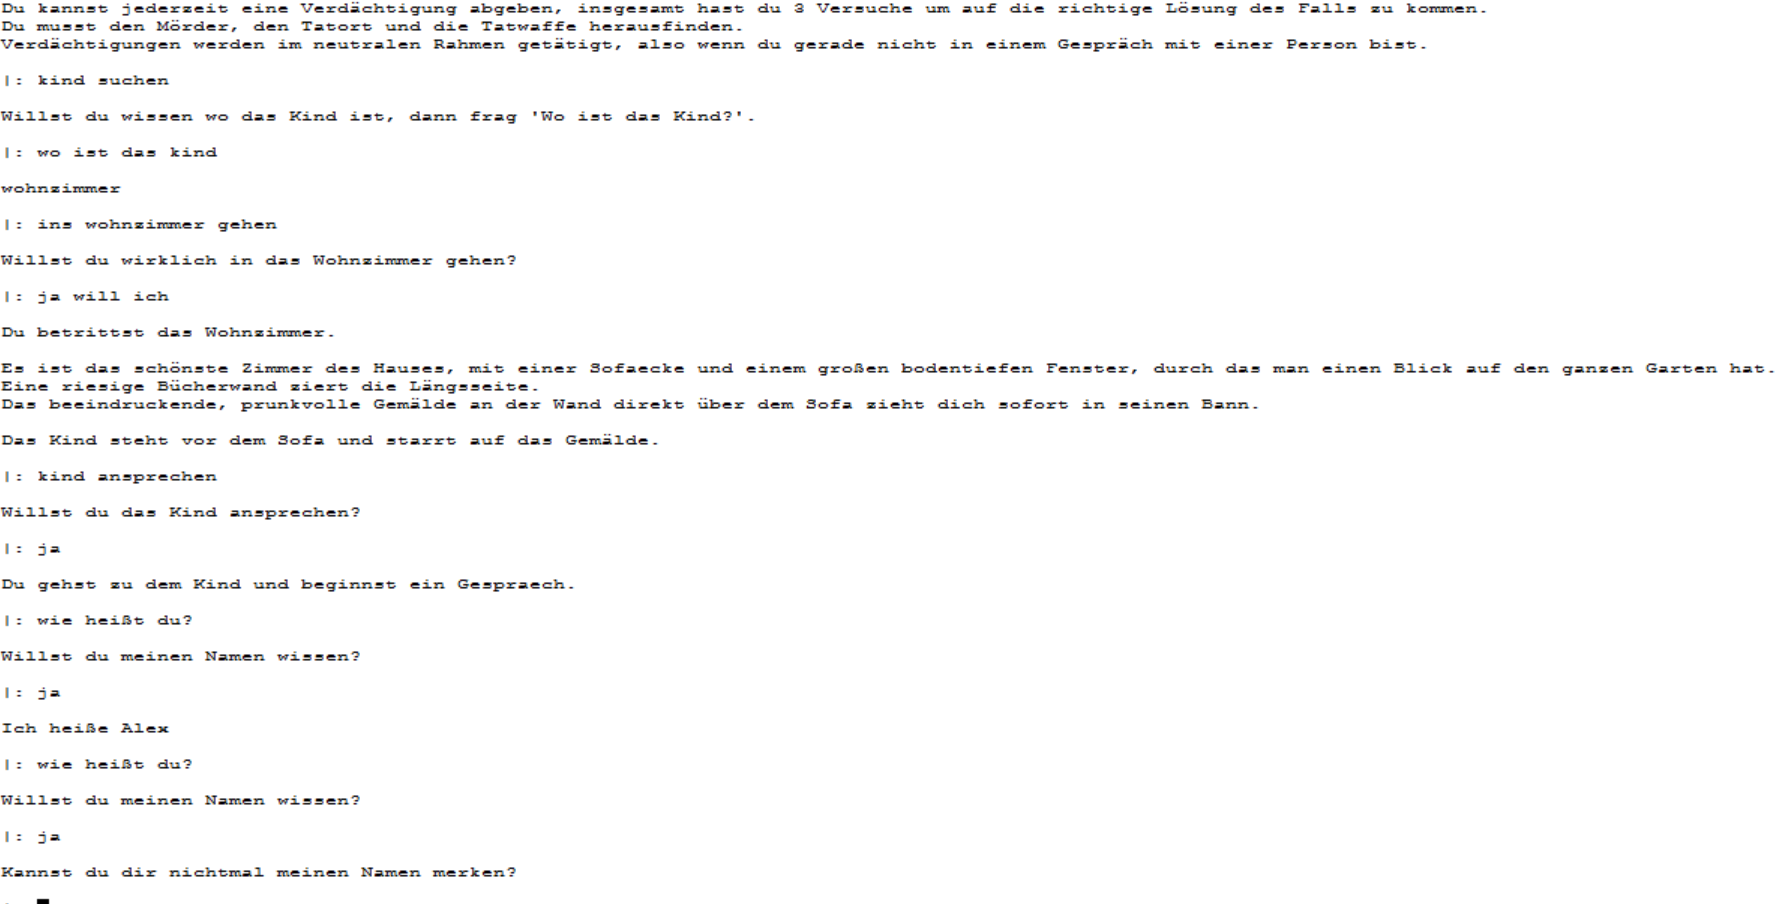
\includegraphics[scale=0.7]{bild1.png}
\end{minipage}\\
\begin{minipage}{0.5\textwidth}
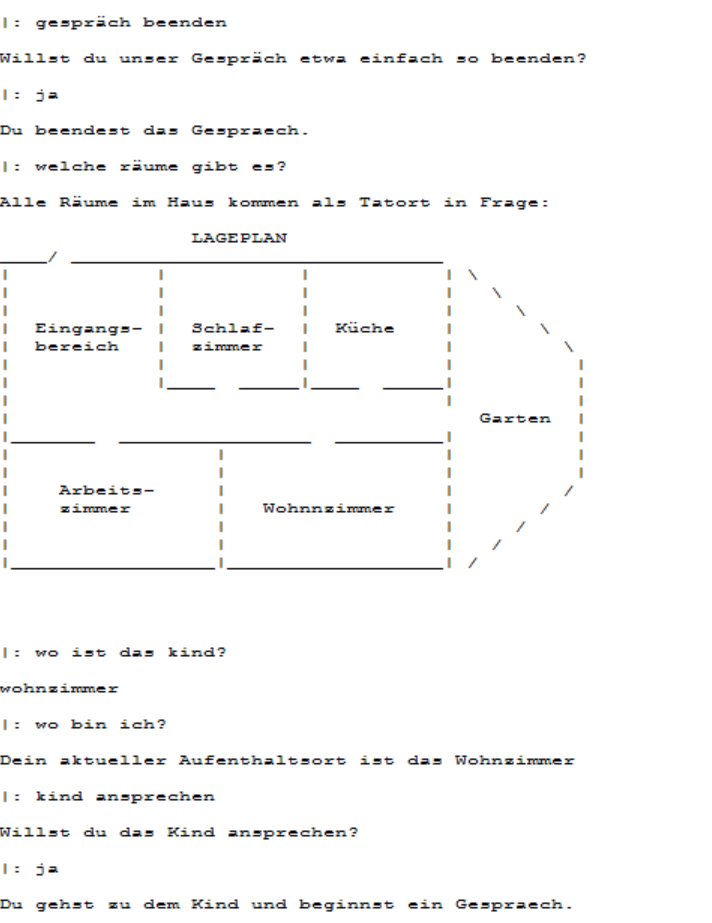
\includegraphics[scale=0.7]{bild2.png}
\end{minipage}\\
\begin{minipage}{0.5\textwidth}
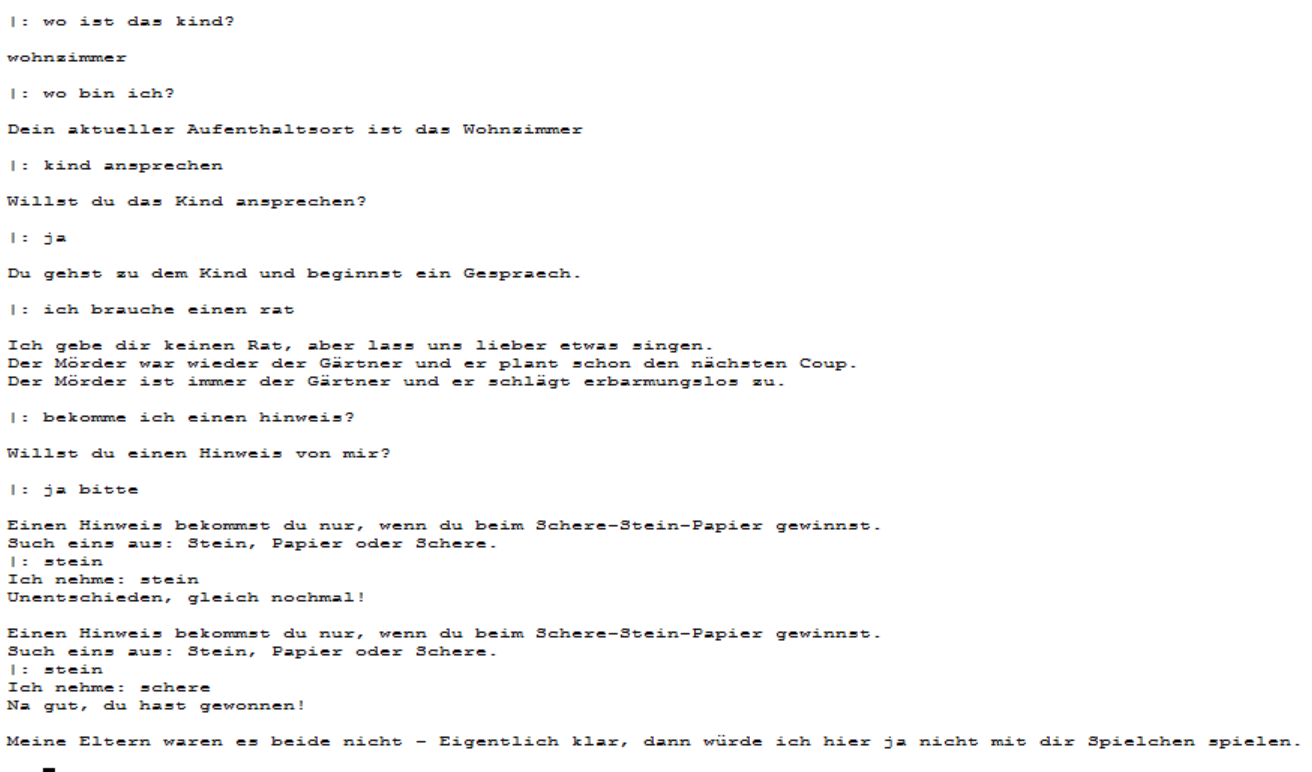
\includegraphics[scale=0.7]{bild3.png}
\end{minipage}

\end{itemize}


VIEL SPAß BEIM SPIELEN!




\end{document}

